\chapter{Exercise 1}
\label{sec:ugeopgave-1}

The purpose of this exercise is to give a short introduction to create, edit, link and run C/C++ programs that are based on the graphics library OpenGL, and the utility libraries Angel and GLUT.

\section{Part 1}
\label{sec:del-1}

I have added the duties and meanings of functions as comments in source file.\\
The extra white triangle can be seen in Figure \ref{fig:1-1-1}.

\begin{figure}[hp]
\centering
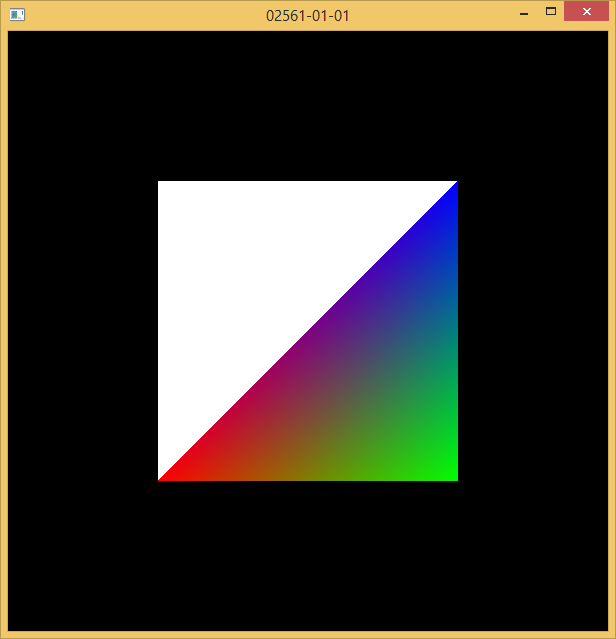
\includegraphics[width=8cm]{../Screenshots/ex-1/1.png}
\caption{White Triangle}
\label{fig:1-1-1}
\end{figure}


\section{Part 2}
\label{sec:del-2}

I understand the overall structure of the program. I extend the the program with a red triangle according to given description. Then I translate the triangle with the vector (6,7,0) by modifying modelView-matrix. I define the colors of the vertices accordingly. Finally I rotate the rectangle 45 counter-clockwise around its middle point. The result is captured by a screenshot, given in Figure \ref{fig:1-2-1}.

\begin{figure}[hp]
\centering
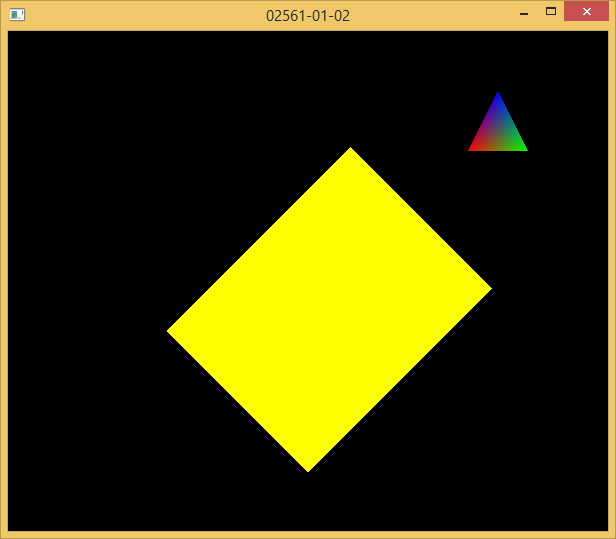
\includegraphics[width=8cm]{../Screenshots/ex-1/2.png}
\caption{Resulting scene}
\label{fig:1-2-1}
\end{figure}


\section{Part 3}
\label{sec:del-3}

\begin{itemize}
  \item glDrawArrays uses vertices in given order. Unlike glDrawArrays, glDrawArrays can use the vertices array elements in any order.
  \item GL\_TRIANGLES: Draws triangles on screen. Every three vertices specified compose a triangle.\\
GL\_TRIANGLE\_STRIP: Draws connected triangles on screen. Every vertex specified after first three vertices creates a triangle.\\
GL\_TRIANGLE\_FAN: Draws connected triangles like GL\_TRIANGLE\_STRIP, except draws triangles in fan shape.
\end{itemize}
%
You can see resulting screenshot of extension in Figure \ref{fig:1-3-1}.

\begin{figure}[hp]
\centering
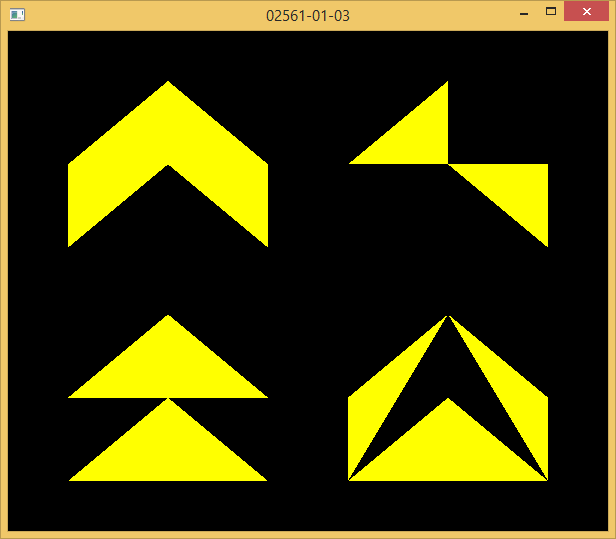
\includegraphics[width=8cm]{../Screenshots/ex-1/3.png}
\caption{Yellow Triangles}
\label{fig:1-3-1}
\end{figure}

\section{Part 4}
\label{sec:del-4}

You can see resulting screenshot of extension in Figure \ref{fig:1-4-1} 

\begin{figure}[hp]
\centering
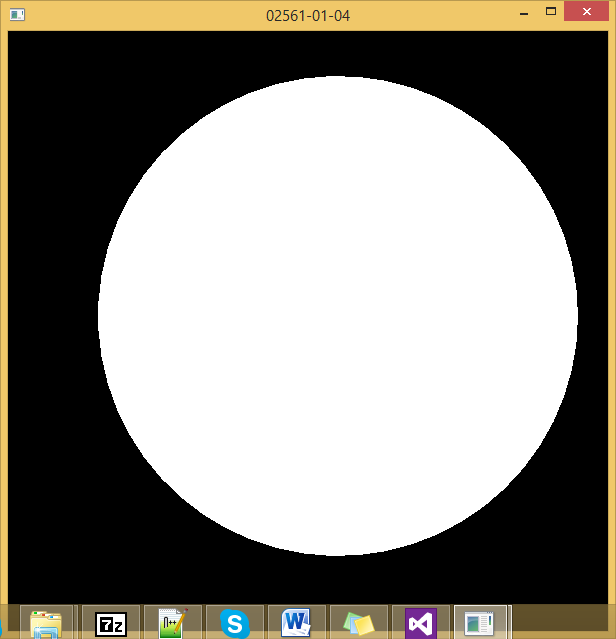
\includegraphics[width=8cm]{../Screenshots/ex-1/4.png}
\caption{A (not a perfect) Circle}
\label{fig:1-4-1}
\end{figure}

\section{Part 5}
\label{sec:del-5}

Instead of changing vertex positions and colors, by making necessary model transformations (like scaling, rotating, translating...) I manage to get the result. You can see the result in Figure \ref{fig:1-5-1}.
 
\begin{figure}[hp]
\centering
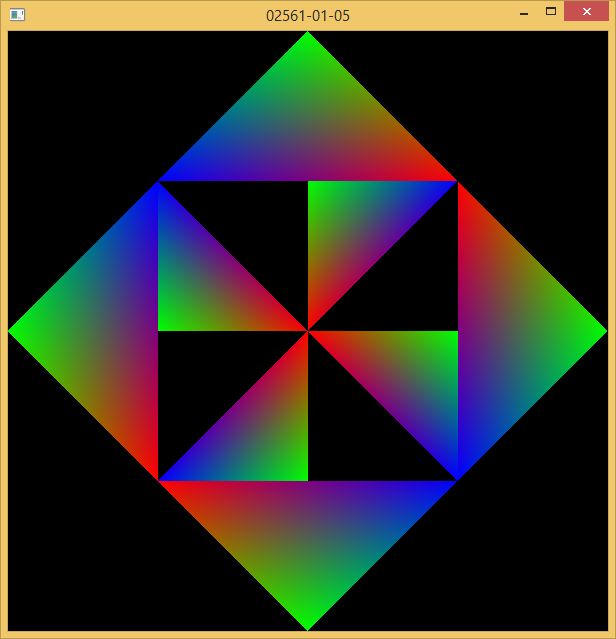
\includegraphics[width=8cm]{../Screenshots/ex-1/5.png}
\caption{After eight times drawing with different model matrices, resulting scene.}
\label{fig:1-5-1}
\end{figure}


\section{Part 6}
\label{sec:del-6}


\begin{itemize}
  \item 



\begin{align*}
  M = & \begin{bmatrix}
          \dfrac{xv2 - xv1}{xw2 - xw1} & 0 &
          -xw1 \cdot \dfrac{xv2 - xv1}{xw2 -
            xw1} + xv1 \\
          0 & \dfrac{yv2 - yv1}{yw2 - yw1} &
          -yw1 \cdot \dfrac{yv2 - yv1}{yw2 -
            yw1} + yv1 \\
          0 & 0 & 1
        \end{bmatrix}
\end{align*}

  \item 
\begin{align*}
  M = & \begin{bmatrix}
          1 & 0 & xv1 \\
          0 & 1 & yv1 \\
          0 & 0 & 1
        \end{bmatrix} 
& \begin{bmatrix}
          \dfrac{xv2 - xv1}{xw2 - xw1} & 0 & 0 \\
          0 & \dfrac{yv2 - yv1}{yw2 - yw1} &  0 \\
          0 & 0 & 1
        \end{bmatrix} 
& \begin{bmatrix}
          1 & 0 & -xw1 \\
          0 & 1 & -yw1 \\
          0 & 0 & 1
        \end{bmatrix} 
\end{align*}
Multiplication of these matrices gives the same result above. 
\end{itemize}

\section{Part 7}
\label{sec:del-7}

The pictures below 
Figure \ref{fig:1-7-1}, 
Figure \ref{fig:1-7-2}, and Figure \ref{fig:1-7-3} show the result for 1, 2 and 3 iterations respectively.

\begin{figure}[hp]
\centering
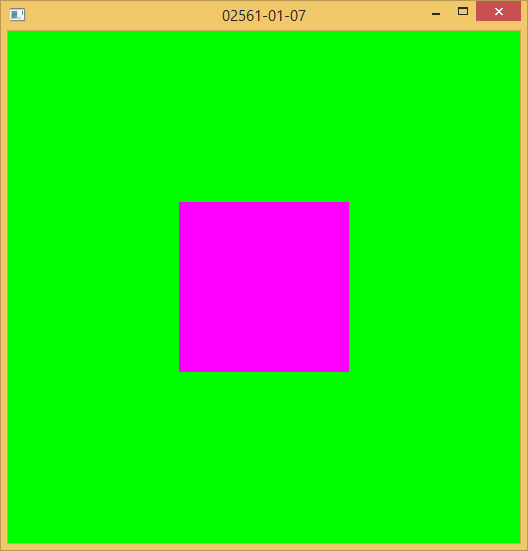
\includegraphics[width=8cm]{../Screenshots/ex-1/7-1.png}
\caption{One iteration Sierpinski carpet}
\label{fig:1-7-1}
\end{figure}

\begin{figure}[hp]
\centering
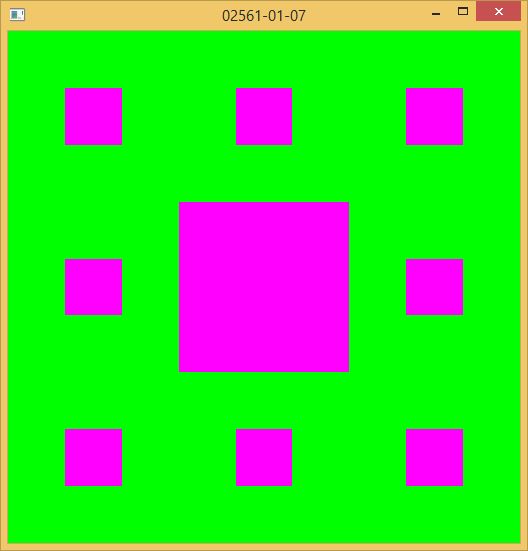
\includegraphics[width=8cm]{../Screenshots/ex-1/7-2.png}
\caption{Two iteration Sierpinski carpet}
\label{fig:1-7-2}
\end{figure}

\begin{figure}[hp]
\centering
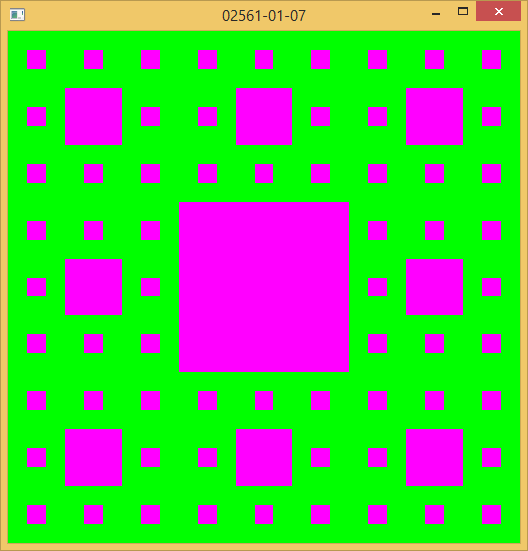
\includegraphics[width=8cm]{../Screenshots/ex-1/7-3.png}
\caption{Three iteration Sierpinski carpet}
\label{fig:1-7-3}
\end{figure}



%%% Local Variables:
%%% mode: latex
%%% TeX-master: "report_main"
%%% End: 